\documentclass[10pt]{article}
\usepackage[polish]{babel}
\usepackage[utf8]{inputenc}
\usepackage[T1]{fontenc}
\usepackage{amsmath}
\usepackage{amsfonts}
\usepackage{amssymb}
\usepackage[version=4]{mhchem}
\usepackage{stmaryrd}
\usepackage{graphicx}
\usepackage[export]{adjustbox}
\graphicspath{ {./images/} }

\title{LIGA MATEMATYCZNA \\
 im. Zdzisława Matuskiego \\
 PAŹDZIERNIK 2022 \\
 SZKOŁA PODSTAWOWA klasy VII - VIII }

\author{}
\date{}


\begin{document}
\maketitle
\section*{ZADANIE 1.}
Wyjeżdżając na wakacje dwudziestu trzech uczniów klasy VII postanowiło pisać do siebie wiadomości tekstowe. Pewnego dnia każdy z nich wysłał dwie lub cztery wiadomości. Czy każdy uczeń mógł tego dnia otrzymać dokładnie trzy wiadomości?

\section*{ZADANIE 2.}
Znajdź taką liczbę trzycyfrową, żeby po dodaniu do niej 500 otrzymać liczbę czterocyfrową podzielną przez 12, a po odjęciu od niej 500 mieć liczbę dwucyfrową podzielną przez 23.

\section*{ZADANIE 3.}
Pewien szyfr do sejfu składa się z 8 różnych cyfr ułożonych malejąco (od lewej do prawej). Liczba ośmiocyfrowa tworząca szyfr dzieli się przez 180. Jaki to szyfr?

\section*{ZADANIE 4.}
Suma pięciu liczb trzycyfrowych \(\overline{a b c}, \overline{b c d}, \overline{c d e}, \overline{d e a}, \overline{e a b}\) jest równa 3996. Oblicz \(a+b+c+d+e\).

\section*{ZADANIE 5.}
Kwadrat \(A B C D\) o polu 400 podzielono na kwadrat \(K_{1}\) o polu 49 , kwadrat \(K_{2}\) i figurę \(F\). Oblicz obwód figury \(F\).\\
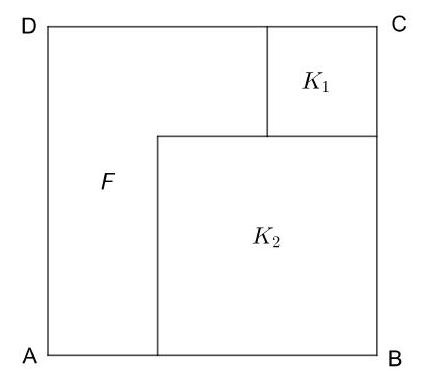
\includegraphics[max width=\textwidth, center]{2024_11_21_f32d77642941077c0701g-1}


\end{document}